\documentclass{acm_proc_article-sp}

\usepackage{amsmath}
\usepackage{verbatim}
\usepackage{textcomp}
\usepackage{graphicx}
\usepackage{subcaption}
\usepackage{url}
\usepackage{multicol}
\usepackage{tikz}
\usetikzlibrary{positioning}
\usepackage{wasysym}
\setlength{\parindent}{1cm}
\usepackage{indentfirst}


\begin{document}

\title{Anonymous Reserve Auction Revenue Bounds \\
{\normalsize Code available at: \url{https://github.com/blasch/AnonymousReserve}}} 
\subtitle{}

\numberofauthors{2} 
\author{
% 1st. author
\alignauthor 
Robert Schneidman \\
	\affaddr{260476707}
% 2nd. author
\alignauthor Benjamin La Schiazza\\
	\affaddr{260531181}
% 3rd. author
}

\date{Nov30}

\maketitle
\begin{abstract}

\end{abstract}

\section{Introduction}
Auction theory is an incredibly relevant field to investigate as it has many modern applications. Society has been running auctions for centuries yet only now with advances in computing technology and mathematics have they been explored in an academic setting. A number of fundamental results have emerged from applying mathematical models to these settings. While some results are incredibly practical and have shaped business models, others remain inapplicable due to their inherent assumptions. 

One of these assumptions involves the nature of the distributions bidders choose they value for an object from. A very common practice is to assume all bidders pick values from the same distribution. In modern auctions settings found especially on the internet, bidders can come from a range of cultures and demographics and makes the applicability of theory stemming from these results not practical. Another fact in the basic auction revenue theory (eg. Myerson's Lemma[1]) is that to achieve optimal revenue, bidders must be assigned bidder specific reserves[2]. While this may be feasible when all bidders have identical distributions (meaning their reserves turn out to be the same), in realistic settings with multiple distributions, it is hard to justify to real bidders that certain participants have a lower or higher reserve to meet to be eligible in the auction. In the name of fairness, though to the determinant of obtaining optimal revenue, real auctions (eg. Ebay) employ a general reserve for all participants. Some general bounds have been noted regarding the approximation of optimal revenue with anonymous reserves but they are not tight\cite[p. 126]{hartline}. 

Due to the prevalence of Anonymous reserve auctions it is important to understand what kind of performance can be expected from their utilization. Our goal with this project was to explore and try and improve guarantees made on the optimal revenue approximations. More specifically, we aim to improve the upper bound proposed by Hartline (Lemma 4.17)\cite{hartline}. If a setting can be found under which the max revenue for anonymous reserve is significantly under 50\% then the possibility of formally improving the bound is there. The simplest setting we can do our investigation under is an auction with one item and two bidders.

\section{Theory}
Our ultimate goal is to make statements about the nature of the revenue one can expect when running a single-item Vickrey auction with an anonymous reserve. The bayesian optimal auction is used as a benchmark. It is appropriate however to lay some foundation before discussion the problem at hand.

\subsection{Dominant Strategy Incentive Compatible}
An auction is Dominant Strategy Incentive Compatible (DSIC) if bidding truthfully is the single strategy that will maximizes a bidder�s utility. If an auction is DSIC, bidding truthfully will never result in a bidder having a negative utility function.

\subsection{Virtual Value}
Myerson showed in 1981 that in a single dimensional setting, given a set of distributions Fi for each bidder, the expected revenue from a DSIC [5] mechanism is 
\[ E[\sum_{i} p_{i}(v)] = E[\sum_{i} x_{i}(v)\phi_{i}(v_{i})] \] \\
where for bidder i and his distribution F,
\[ \phi(v) = v - \frac{1-F(v)}{f(v)}\] \\
$phi_{i}(v)$ is bidder i's \emph{virtual value} function. In order to optimize revenue, a mechanism should allocate goods according to the virtual value function.

\subsection{Vickrey Auction}
A Vickrey auction is an auction where the winner is the bidder with the highest bid but only pays the second highest price once he wins. This auction has a number of desirable properties including incentives for truthful bidding and maximization of general social welfare. [7] It is the mechanism of choice for optimizing revenue. 

\subsection{Single-Item Vickrey Auction with Anonymous Reserve}
A single-item Vickrey auction with anonymous reserve is an auction where the winner is the bidder with the highest bid under the condition that he meets his reserve. He pays the maximum of his reserve price and the second highest bid. This auction is dominant strategy incentive compatible.

\subsection{Single-Item Bayesian Optimal Auction}
The single-item Bayesian optimal auction is an auction where the winner is the bidder with the highest virtual value under the condition that he meets his reserve.  The bidder specific reserve price is set at \[ r = \phi_{i}^{-1}(0)\] for each bidder i in order to maximize virtual welfare (that in turn maximizes expected revenue). The winning bidder pays the maximum price he would need to bid in order to no longer win the auction. This auction is dominant strategy incentive compatible. [7] It is the mechanism of choice for optimizing revenue. 

\subsection{Regular Distributions}
Another point to look at is the nature of the distributions bidders can bid from. While realistically there can be a wide range of distributions for bidders that my not align well with idealized functions, it is safe to focus on a set of distributions with nice properties. The distributions we will explore are called Regular distributions and are defined as functions whose virtual value functions are non-decreasing. When all bidder's distributions are regular, the mechanism maximizing virtual welfare is monotone. [WHY IMPORTANT??]

Common distributions in this class include the normal distribution, exponential distribution and uniform distribution. Some equally interesting distributions are "fat-tailed" distributions, defined as having a probability distribution \\
\[  f(x) \sim x^{-(1 + \alpha)} \: as \: x \rightarrow \infty ,\: \alpha > 0 \] \\
Since we are looking to show a worst-case bound on the revenue in an arbitrary anonymous reserve auction with regular bidders, we want to investigate the "least regular" function in this class, the equal-revenue distribution [8]. It's probability distribution is an instance of a fat-tailed distribution and is as follows, \\
\[  f(x) = \frac{1}{x^2} \] \\
It lies on the boundary of regularity as it's virtual value function is flat.

\subsection{Anonymous Reserve Approximation of Optimal Revenue}
As discussed, to get the optimal revenue in a two bidder-one item auction one needs to assign a bidder specific reserve. In an idealized setting this is perfectly acceptable but certainly not justifiable in practice. Anonymous reserves are a means to keep the auction process fair for all bidders. But how does the expected revenue change compare to the optimal revenue had we foregone fairness? Is there a way to set the anonymous reserve to maximize revenue and in the worst case what are the approximations for the optimal revenue?

In Hartline's book draft \cite{hartline}, Lemma 4.18 and Theorem 4.19 state that in the worst case, given arbitrary regular distributions, an anonymous reserve auction will yield between 25\% and 50\% of the optimal revenue. Without detailing the proofs themselves, in the case of Lemma 4.18 (the upper bound), Hartline makes use of the equal-revenue distribution as detailed above because it is on the border of regularity. 

Beyond Hartline's exploration of the topic, there does not seem to be any other research into the revenue bounds of anonymous reserves despite it's relevance to many business models in various spaces.

\section{Methodology}
Our approach to explore this topic was by simulation. By setting up an auction between various types of bidders, calculating the expected revenue under anonymous reserves and the optimal revenue, we can search for situations were the ratio of anonymous reserve revenue to optimal revenue is under 50\%.

\subsection{Bidder Distributions}
The pool of bidders used to set up auctions was populated with bidders with the following underlying regular distributions for their values: uniform, exponential, gamma, normal, equal revenue distribution (ERD), fat-tailed distributions with alpha equal to two, three and four and finally a bidder that always bids 1. 

Due to the way the distributions are encoded, we generate a sample of size 10000 produced by sampling each distribution. This becomes the "sample space" of the distributions and is what we use when searching over bidder values. This is the main reason why results are not exactly consistent over many runs. The deviation observed however is not significant.

\subsection{Experimental Set-up}
The space of auctions investigated were that of one item with two bidders. To begin, Hartline�s proof of a 50\% approximation was the most appropriate place to start (bidder that always bids 1 and an ERD bidder) After that we pair up each distribution from our pool with a bidder bidding with the ERD. Since the ERD is borderline regular, intuitively the most sub-optimal cases will be found along this boundary. Inspired by the direction the formal proof took involving one of these bidders, we took the same approach.

\subsection{Setting Bidder Specific Optimal Reserves}

Initially, the process of finding the  bidder specific reserve was done by an exhaustive search method. All values x where 0 < cdf(x) < 1 were tested in order to maximize the single item single bidder posted price revenue. The calculation was done this way because many distributions do not have a closed form solution for finding $\phi^{-1}(0)$. Eventually, the process of setting a bidder specific reserve was done using a library function which was able to solve for $\phi^{-1}(0)$. This change allowed us to reduce the error when calculating the optimal revenue since the search increments were not infinitesimally small.

\subsection{Setting Anonymous Reserves}

	Due to the large number of iterations of each auctions that were run, sacrifices had to be made in terms of discretization of candidate reserves. The intervals between anonymous reserves that were tested was proportional to the range of bidder valuations. This was the most logical portion of the program to sacrifice precision. In most cases, a sub-optimal anonymous reserve exceeded the 50\% approximation (with error accounted for). In the case where the 50\% approximation was not met, the auction was tested a subsequent time with smaller intervals used to pinpoint the anonymous reserve. 
 
\subsection{Running Auctions}

After the reserve price was set, each auction was run proportional to the minimum probability of each bidder bidding above the reserve price (will be easier to understand when formula is written). A factor of 1000 was applied to reduce the error. No auction was run more then 10,000 times due to run time constraints. Under these conditions, a conservative error approximation of 10\% by comparing the experimental revenues with the theoretical expected revenue.  Under this 10\% error for both the optimal and anonymous reserve auctions, all auctions that approximated the optimal revenue less then 66.66\% were considered for re-testing.

With the Optimal reserves fixed for each bidder and the anonymous reserve found, the optimal Bayesian auction and a Vickrey auction with anonymous reserve are run over a sample space of the respective distributions of the bidders. This allowed us to collect data regarding the expected revenue under a range of anonymous reserves and the best approximation of the optimal revenue.

\section{Results}

The results of our experimentation were in general not very surprising. The ratio of the max expected revenue under anonymous reserve to optimal revenue for these two bidder auctions varied between 50\% to ~90\%. 

\subsection{Hartline's Proof}

As stated earlier, our first challenge was validating Hartline's theoretical argument that he used in the proof of the upper bound \cite[p. 126]{hartline}. The setting is a two bidder auction with one bidder with an underlying ERD and the other always bidding 1. Figure \ref{fig:proofgraph} shows the result of a Vickrey auction with many anonymous reserves. Accounting for experimental error, the results are as stated in the formal proof, the expected revenue hovers around 1 (max of 1.06 used for ratio).

 	\begin{figure}[!htbp]
   		\centering
  		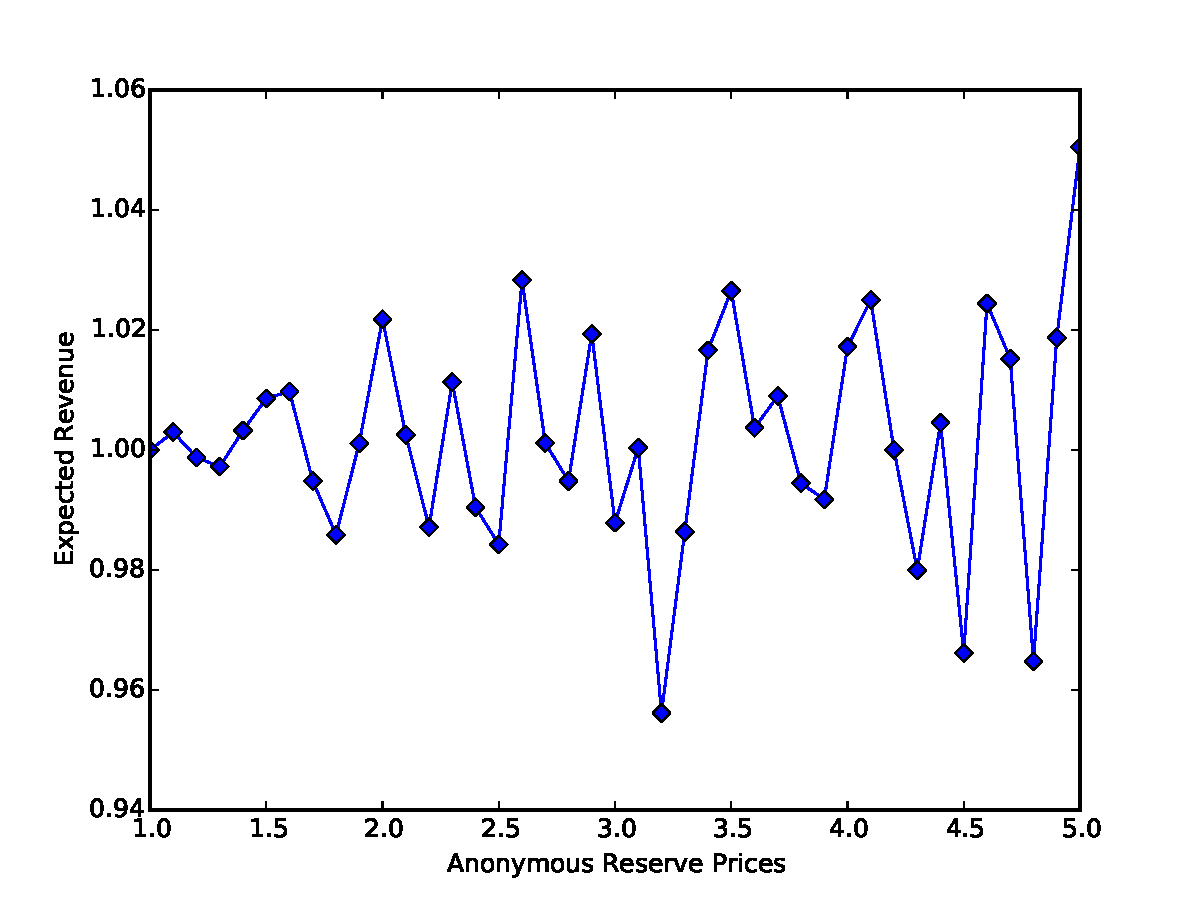
\includegraphics[width=\linewidth]{0_1_0.pdf}
    		\caption{Expected revenue for proof setting over anonymous reserves.}
    		\label{fig:proofgraph}
	\end{figure}
	
The optimal revenue calculated in the experiment was 2.0197 (very much in line with the theoretical 2 shown in the paper \cite{hartline}). The ratio is evidently ~0.52. Many runs shows that the ratio does indeed hover around 0.5, confirming the proof of the upper bound given in Hartline's book.

\subsection{Did we do better?}

Unfortunately this was the closest any of our simulated auctions got to the upper bound proposed. All other scenarios had ratios well closer to 1 of the optimal revenue. In fact all of the other pairings with an ERD produced (within error) a ratio around 1. One to highlight is an auction between two ERD. As they have identical distributions, the ratio was ~1 with Figure \ref{fig:erd2} showing data collected for anonymous reserve auction. The optimal expected revenue is theoretically 2 and the anonymous auction achieves approximately the same result.

	\begin{figure}[!htbp]
   		\centering
  		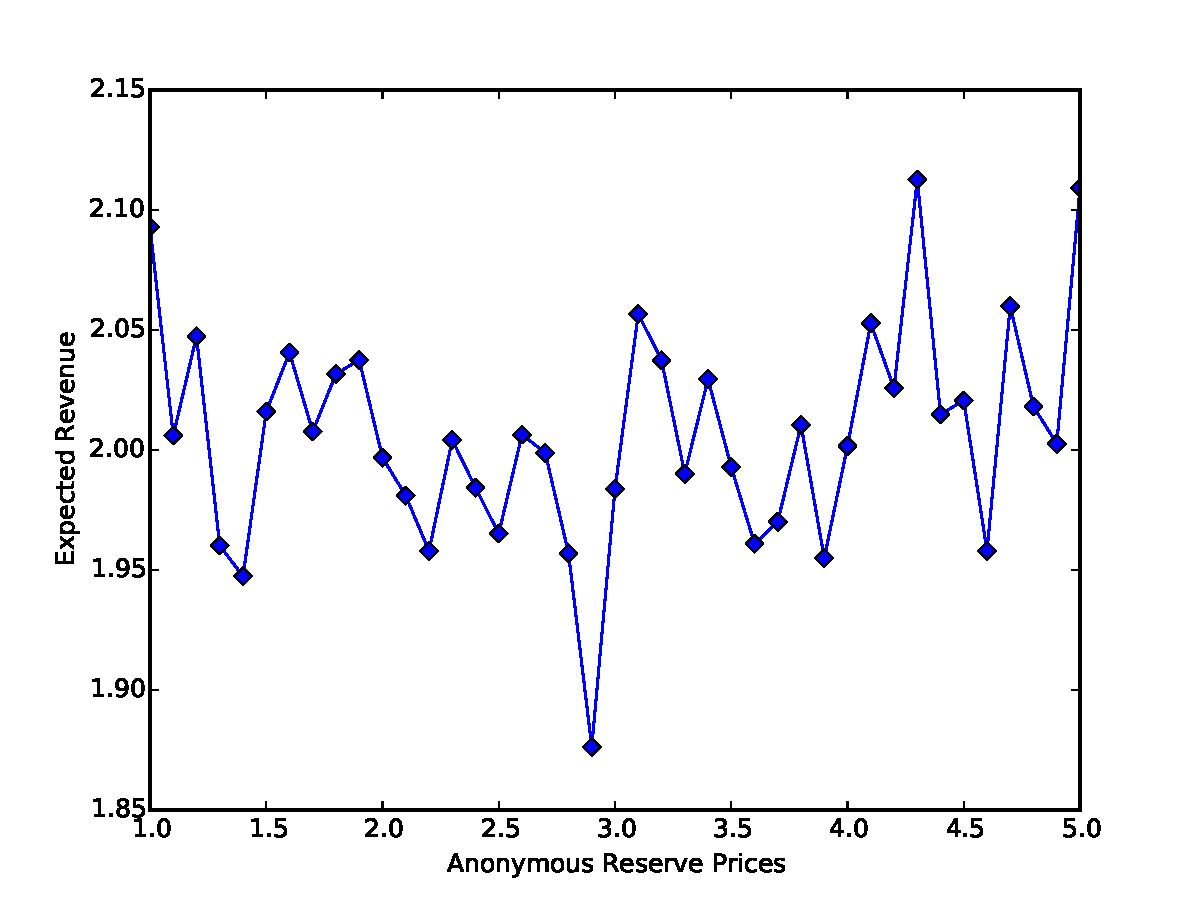
\includegraphics[width=\linewidth]{0_1_5.pdf}
    		\caption{Expected revenue over anonymous reserves.}
    		\label{fig:erd2}
	\end{figure}

\section{Discussion}

The results were clearly not very groundbreaking. The theoretical proof was re-implemented successfully and a large number of similar auctions involving a range of regular distributions were run. All the other results had approximations of the optimal revenue hovering around 100\%.

\section{Conclusion}

\begin{thebibliography}{9}

	\bibitem{hartline}
		"4 Bayesian Approximation." Mechanism Design and Approximation. N.p.: n.p., n.d. N. pag. Jason Hartline. N/A. Web. 6 Dec. 2014. <http://jasonhartline.com/MDnA/MDnA-ch1to6.pdf>.

\end{thebibliography}

\end{document}
